\documentclass[12pt]{amsart}
\usepackage{amsmath, amsthm, amssymb, graphicx, setspace, listings, float, hyperref}
\usepackage[margin=1in]{geometry}
%You will want the setspace.sty file in the same folder as your source file when you use this template

%Sets the margins

%\textwidth = 6.5 in
%\textheight = 9 in
%\oddsidemargin = 0.0 in
%\evensidemargin = 0.0 in
%\topmargin = 0.0 in
%\headheight = 0.0 in
%\headsep = 0.0 in
%\parskip = 0.2in
%\parindent = 0.0in

%defines a few theorem-type environments
\newtheorem{theorem}{Theorem}
\newtheorem{corollary}[theorem]{Corollary}
\newtheorem{definition}{Definition}

\title{Machine Learning LAB 01}
\author{Stefano Fochesatto}
\date{\today} % Uncomment and insert a date to specify a date

%%% BEGIN DOCUMENT
\begin{document}


\doublespacing %%INCLUDE THIS TO DOUBLESPACE!


\maketitle
%\renewcommand{\baselinestretch}{1.2}

\section{Introduction}%Change what's in brackets to change the section title.
In this lab we will build a CART model to detect whether or not an email is spam. In doing so we will 
explore SPM's CART Decision Tree Analysis Engine, and develop a data workflow with SPM. The data used throughout this lab 
can be found on Kaggle and is free to use for educational purposes under the Open Data Commons Open Database License.
The data comes in the form of a .csv file with 5172 rows and 3002 columns. Each row represents data for a single email, the first 
column is used to number each email, the last column contains our prediction information(1 for spam, 0 for not spam) and the rest of the columns
contain word counts for the 3000 most common words found across all emails. \\\\


\subsection*{Preliminary Analysis (Loading Data)}
Upon loading the data into SPM using either the file menu, or the USE"" command, we are met with a variety of options 
to perform exploratory analysis and data preparation in the 'Activity' pane. For the most part the most important tools for 
exploratory analysis are the View Data, Stats, Graphs, and Correlation options in this menu (these options can also be found under 
ther View and Explore menues). With these options we can view histograms, 
evaluate correlations, and compute univariate statistics like the Mean, Min, Max and IQR. Not entirely relevant to 
our lab but usefully nonetheless. \\
\begin{figure}[H]
    \begin{center}
    \caption{SPM Activity Pane}
    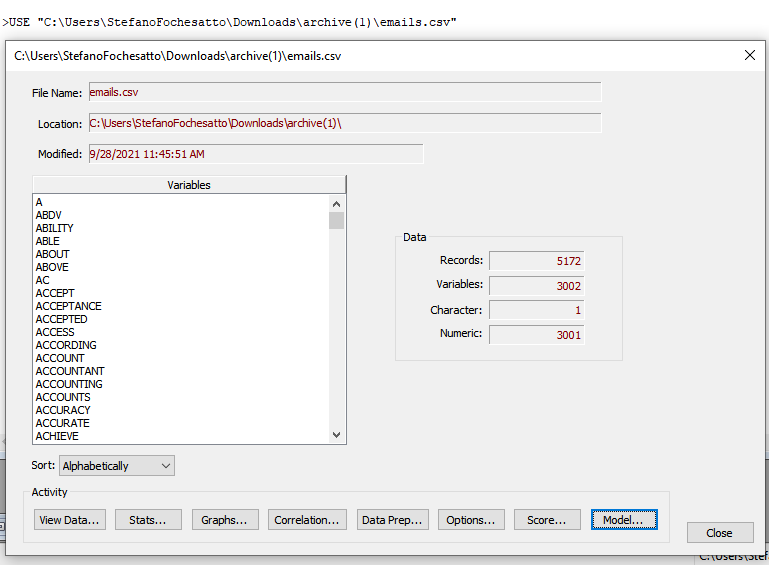
\includegraphics[width=.75\linewidth]{fig1.png}
    \end{center}
    \end{figure}

The Data Prep option allows us to do any preparation like handling missing data, duplicate data, unwanted outliers, or even 
fixing structural errors in our data using built in SPM commands. The Options menu gives us access to the content of our Model's text
report, as well as the random number seeds for each SPM modeling engine. 
\section{SPM CART Model}


\section{Performance Analysis}


\section{Conclusion}




\end{document} 
















